\section{Experimental Evaluation}\label{sec:exp-evaluation}
We evaluated the above mentioned greedy heuristics based approach in a Apache Spark. Spark's SQL optimizer allows passing the optimizer rules externally to the application. We implemented an optimizer which takes the optimized plan as input and based on the heuristics proposed, reorders the joins wherever applicable . It is assumed that the table sizes are available in the Spark optimized plan before applying this rule. We used the TPC DS dataset (scale 100) non-partitioned dataset for evaluating the performance. The experiments were ran on a 5 node Apache Spark cluster on AWS with machine type r4.4xlarge.

Out of 100 TPC-DS queries, we were able to reorder at least one join in the 38 queries. For the queries not reordered, the performance would be same as before. Figure 4 shows the runtime of few of the queries with and without the optimisation. We saw approximately 26\% improvement in the reordered queries and no performance degradation in any of the reordered query.

\begin{figure}[ht]
\centerline{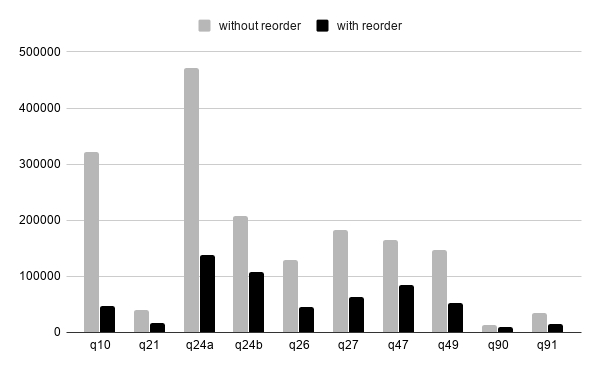
\includegraphics[width=7cm]{fig/chart.png}}
\caption{Performance reordered sample queries}
\label{performance_number}
\end{figure}